\documentclass[a4paper,10pt]{article}

\usepackage{ucs}
\usepackage[utf8]{inputenc}
\usepackage{amsmath}
\usepackage{babel}
\usepackage{fontenc}
\usepackage{graphicx}
\usepackage{textgreek}
\usepackage{subcaption}

\usepackage{hyperref}

\date{12/08/2019}

\begin{document}
 
 \subsection{ensemble di reti neurali}
 Una rete di dimensioni finite raramente apprende completamente un particolare mapping e pu\'o generalizzare male. Aumentare la dimensione o il numero di hidden layer per\'o, il pi\'u delle volte, non porta a nessun miglioramento (Soulie, 1987) anzi, aumentando la dimensionalit\'a del problema aumenta la possibilit\'a che la rete si stabilizzi lontana dalla soluzione desiderata. 
 Molti ricercatori hanno dimostrato che la semplice combinazione degli output di molti classificatori pu\'o generare previsioni pi\'u accurate di quelle di qualsiasi classificatore (Clemen 1989; Wolpert 1992). In particolare, la combinazione di reti neurali addestrate separatamente (comunemente indicato come ensemble di reti neurali) si \'e dimostrata particolarmente efficace (Alpaydin 1993; Drucker et al. 1994; Krogh e Vedelsby 1995; Maclin e Shavlik 1995; Perrone 1992). 
 Figura \ref{EnsembleStructurepng} illustra la struttura generale di un ensemble di reti neurali. Ogni rete nell'ensemble \'e per prima cosa addestrato e poi, per ogni esempio del training, l'output predetto di ognuna delle reti \'e combinato dal judge per produrre l'output dell'ensemble. 
 \begin{figure}[h!]
  \centering
  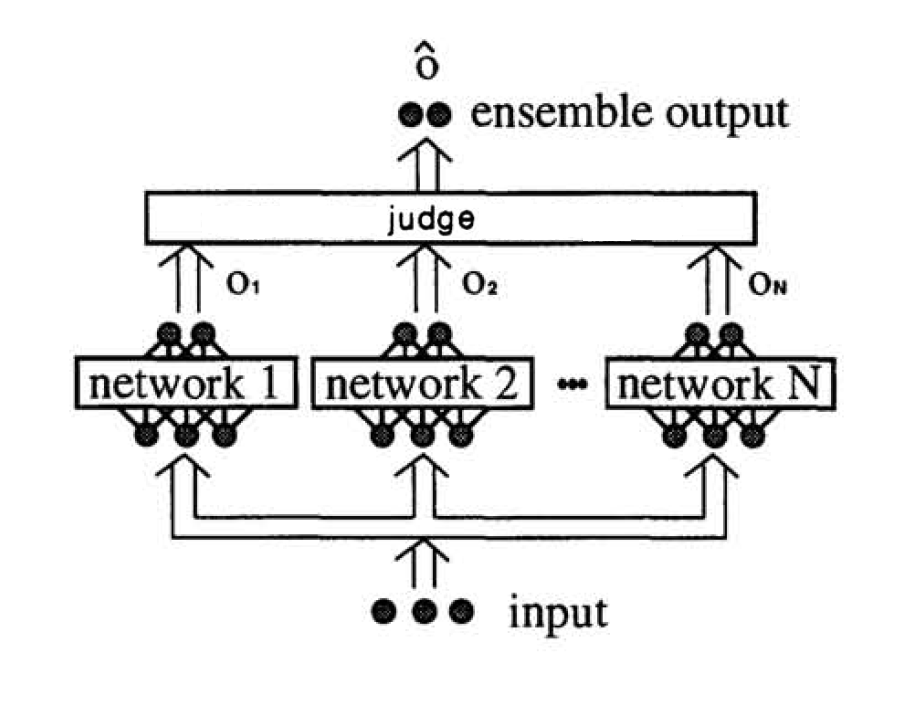
\includegraphics[scale=0.3]{EnsembleStructure.png}
  \caption{da inserire}
  \label{EnsembleStructurepng}
 \end{figure}
 
 L'output dell'ensemble pu\'o anche essere utilizzato come ulteriore training restituendolo alle singole reti. Infatti, nel caso in cui nell'ensemble vi siano una o pi\'u reti poco efficienti e non si hanno a disposizione pi\'u esempi per il training, si pu\'o utilizzare l'output dell'ensemble come output desiderato nelle seingole reti per continuare l'addestramento (aggiungere riferimento). 
 L'errore di una singola rete dipende dalle dimensioni del hidden layer e dalla durata del training. Tuttavia in generale l'errore non \'e una funzione decrescente della dimensione dell'hidden layer. In figura \ref{NetErrHiddenLapng} e \ref{NetErrHiddenLbpng} si mostra l'errore di una singola rete rispetto alla dimensione dell'hidden layer per diversi step di training. D'altra parte la miglior capacit\'a di apprendimento di un ensemble dipende, come accennato in precedenza, dalla sinergia tra le singole reti e non dalle maggiori dimensioni rispetto alla singola rete. Questo \'e principalmente ci\'o di cui discutono anche William P. Lincoln e Josef Skrzypek in $Synergy$ $of$ $clustering$ $multiple$ $back$ $propagation$ $networks$, dove confrontano le prestazioni di ogni singola rete con le prestazioni di un enseble di 5 reti neurali, con stessa struttura della singola.
 
 \begin{figure}[h!]
  \centering
  \begin{subfigure}[b]{0.4\linewidth}
   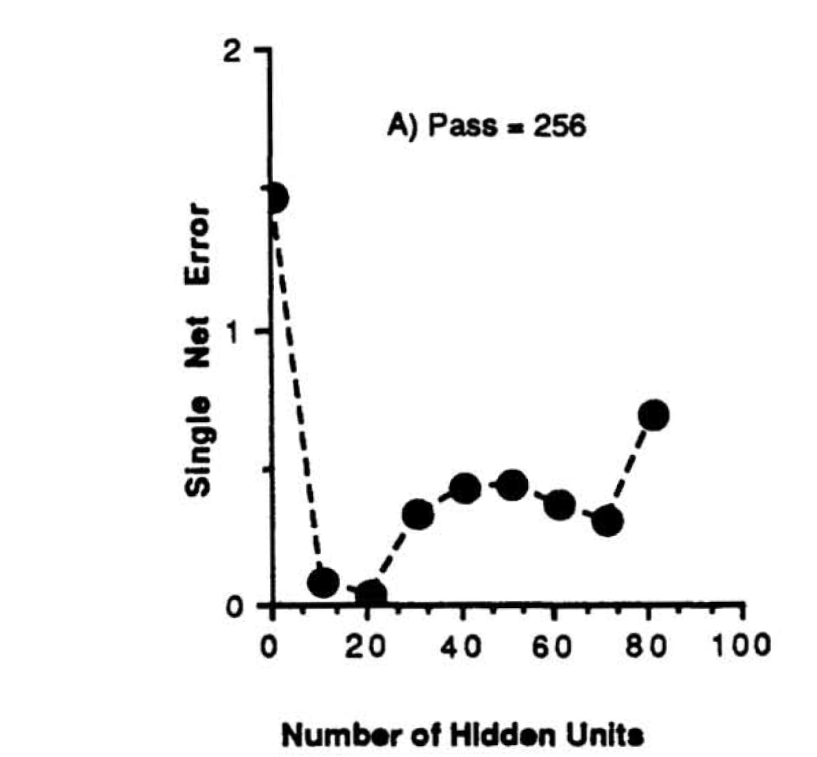
\includegraphics[width=\linewidth]{NetErrHiddenLa.png}
   \caption{da inserire}
   \label{NetErrHiddLapgn}
  \end{subfigure}
  \begin{subfigure}[b]{0.4\linewidth}
   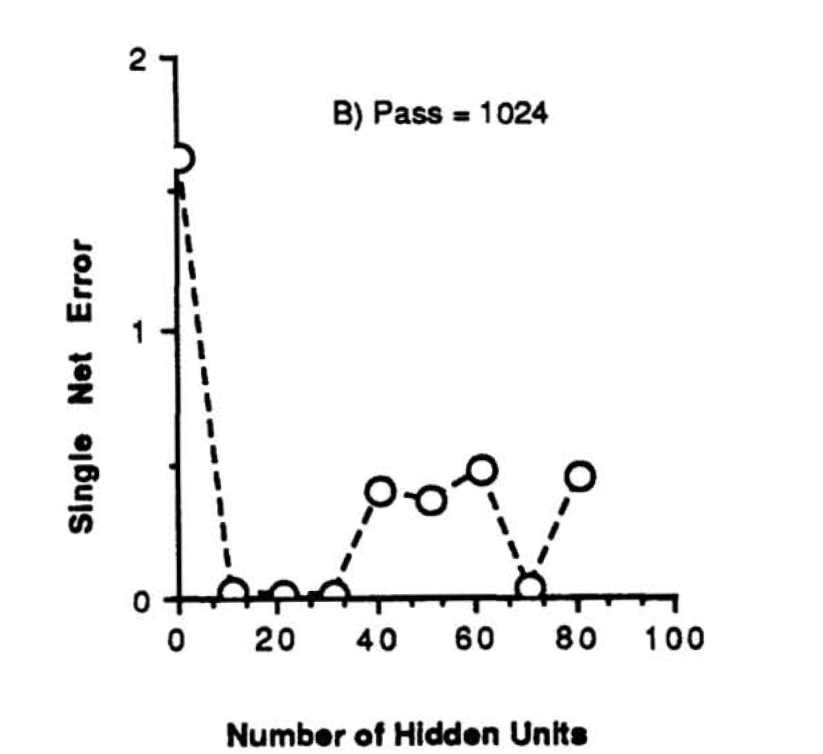
\includegraphics[width=\linewidth]{NetErrHiddenLb.png}
   \caption{da inserire}
   \label{NetErrHiddLbpgn}
  \end{subfigure}
 \end{figure}

 
 Vengono confrontati gli errori medi dei due sistemi. Una misura utile del vantaggio dell'ensemble si ottiene prendendo il rapporto tra l'errore di una singola rete e l'errore del judge. Questo rapporto sar\'a inferiore o maggiore di 1 a seconda del valore assoluto dell'errore della singola rete neurale e dell'ensemble. Figura \ref{EnsembleAdvantageapng} e \ref{EnsembleAdvantagebpng} mostrano il vantaggio dell'ensemble rispetto agli errori della rete singola rispettivamente per 256 e 1024 step del training. Nei casi estremi in cui l'apprendimento sia nullo o quasi totale, l'ensemble non mostra particolari vantaggi, tuttavia si ha un notevole vantaggio se l'apprendimento \'e solo parziale.
 
 \begin{figure}[h!]
  \centering
  \begin{subfigure}[b]{0.4\linewidth}
   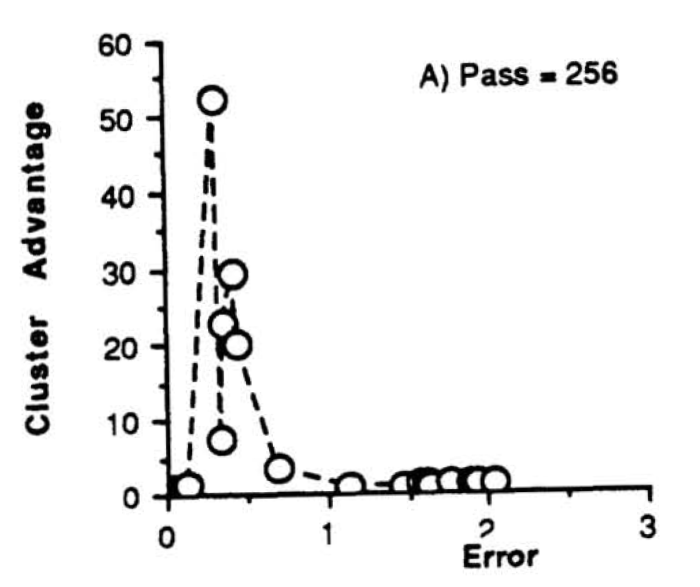
\includegraphics[width=\linewidth]{ClusterErrora.png}
   \caption{da inserire}
   \label{EnsembleAdvantageapng}
  \end{subfigure}
  \begin{subfigure}[b]{0.4\linewidth}
   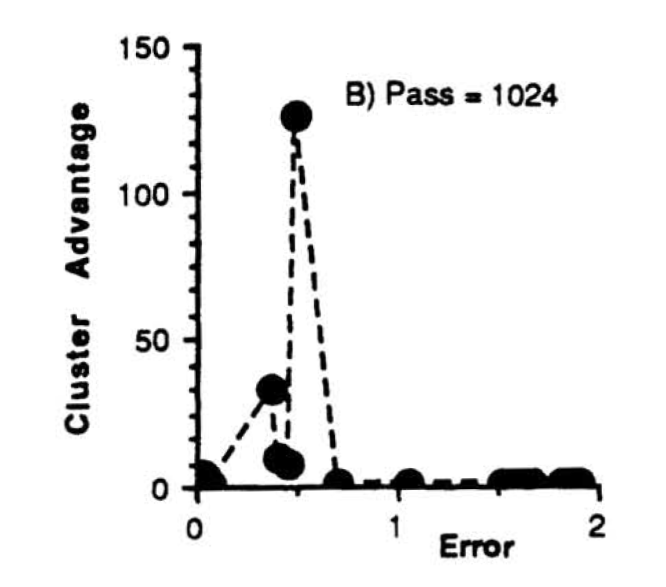
\includegraphics[width=\linewidth]{ClusterErrorb.png}
   \caption{da inserire}
   \label{EnsembleAdvantagebpng}
  \end{subfigure}
 \end{figure}
 
 \subsubsection{judge}
 
 Dato un singolo input, le reti neurali dell'ensemble daranno presumibilmente degli output $Y_k$ diversi, che diventano l'input del $judge$. Quest'ultimo combinandoli ottiene il risultato finale $Y$. Esistono diversi metodi per calcolare $Y$, ma per semplicit\'a consideriamo i due casi pi\'u semplici:
 \begin{align}
  Y &= \sum_{k=1}^N \frac{1}{N} Y_k \\
  Y &= \sum_{k=1}^N W_k Y_k
 \end{align}
 Il primo \'e dato da una semplice media dei $Y_k$, mentre nel secondo caso si considera una media pesata, con i $W_k$ che indicano ``l'affidabilit\'a'' delle singole reti neurali. Seguendo questo ragionamento i $W_k$ vengono di volta in volta modificati come segue:
 \begin{align}
  W_k &= W_k \cdot G \cdot \frac{e}{e_k} \label{JudgeWeights} \\
  e &= \frac{1}{N} \sum{k=1}^N e_k \\
  e_k &= \left | Y - Y_k \right |
 \end{align}
 Con $e$ che indica il tasso di correzione e $e_k$ \'e la deviazione dell'output della singola rete dall'output dell'ensemble.
 
 Dopo il periodo di training iniziale, si presume generalmente che la rete neurale non sia pi\'u soggetta ad ulteriore training. Tuttavia, come gi\'a  anticipato, si pu\'o restituire l'output del judge alle singole reti neurali come output desiderato. William P. Lincoln e Josef Skrzypek in $Synergy$ $of$ $clustering$ $multiple$ $back$ $propagation$ $networks$ affermano che questo procedimento migliori la resistenza al rumore e l'auto-organizzazione $(da capire cosa sia)$.
  
 \subsubsection{ottimizzazione dell'ensemble}
  Precedenti lavori sia teorici (Hansen e Salamon 1990; Krogh e Vedelsby 1995) che empirici (Hashem et al. 1994; Maclin e shavik 1995) hanno dimostrato che un ensemble efficace dovrebbe consistere non solo in reti particolarmente performanti, ma anche in reti che commettano errori in parti distinte dello spazio degli input. 
  Assumiamo che l'obiettivo sia quello di apprendere una funzione $f:R^N\to R$ per la quale abbiamo $p$ coppie input-output per il training con $Y_k = f \left( x_k \right) $ e $k=1, \cdots , p$. L'ensenble consiste in $N$ reti e chiamiamo $V^{\alpha}\left( x\right)$ l'output della rete $\alpha$ relativo all'input $x$. Definiamo nel modo seguente il valore ottenuto dal judge: 
  \begin{equation}
   \overline{V}\left(x\right) = \sum_{\alpha} w_{\alpha} V^{\alpha}\left(x\right).
  \end{equation}
  Consideriamo i pesi $w_{\alpha}$ come l'affidabilit\'a della rete $\alpha$ e di conseguenza li vincoliamo ad essere positivi e normalizzati, cio\'e $\sum_{\alpha} w_{\alpha} = 1$. L'\textit{ambuiguit\'a} su un input $x$ di un singolo membro dell'ensemble \'e definito come $a^{\alpha}\left(x\right)=\left(V^{\alpha}\left(x\right)-\overline{V}\left(x\right)\right)^2$. La \textit{ambiguit\'a dell'ensemble} su un input $x$ \'e data da:
  \begin{equation}
   \overline{a}\left(x\right) = \sum_{\alpha} w_{\alpha} a^{\alpha}\left(x\right) = \sum_{\alpha} w_{\alpha}\left(V^{\alpha}\left(x\right)-\overline{V}\left(x\right)\right)^2. \label{EnsembleAmbiguity}
  \end{equation}
  \'E quindi una varianza e misura il disaccordo delle reti sull'input $x$. L'errore quadratico della rete $\alpha$ e dell'ensemble  sono rispettivamente:
  \begin{align}
   e^{\alpha}\left(x\right) &= \left(f\left(x\right)-V^{\alpha}\left(x\right)\right)^2 \\
   e\left(x\right) &= \left(f\left(x\right)-\overline{V}\left(x\right)\right)^2 \label{ensembleQE}
  \end{align}
  Aggiungendo e sottraendo $f\left(x\right)$ alla \ref{EnsembleAmbiguity} si ottiene:
  \begin{equation}
   \overline{a}\left(x\right) = \sum_{\alpha} w_{\alpha} e^{\alpha}\left(x\right) - e\left(x\right).
  \end{equation}
  Chiamando la media pesata degli errori delle singole reti $\overline{e}\left(x\right) = \sum_{\alpha} w_{\alpha} e^{\alpha}\left(x\right)$ allora la \ref{ensembleQE} diventa:
  \begin{equation}
   e\left(x\right) = \overline{e}\left(x\right) - \overline{a}\left(x\right). \label{GeneralizationError}
  \end{equation}
  Queste ultime formule possono essere mediate lungo la distribuzione degli input, ottenendo le seguenti:
  \begin{align}
   E^{\alpha} &= \int dx \; p\left(x\right) \; e^{\alpha}\left(x\right) \\
   A^{\alpha} &= \int dx \; p\left(x\right) \; a^{\alpha}\left(x\right) \\
   E &= \int dx \; p\left(x\right) \; e\left(x\right).
  \end{align}
  Le prime due sono rispettivamente l'errore generalizzato e l'ambiguit\'a della rete $\alpha$ e $E$ \'e l'errore generalizzato dell'ensemble. Dalla \ref{GeneralizationError} otteniamo:
  \begin{equation}
   E = \overline{E} - \overline{A} \label{EnsembleGeneralizationError}
  \end{equation}
  con $\overline{E} = \sum_{\alpha} w_{\alpha} E^{\alpha}$ la media pesata degli errori generalizzati delle singole reti e $\overline{A} = \sum_{\alpha} w_{\alpha} A^{\alpha}$ la media pesata delle ambiguit\'a delle singole reti.
  Questa equazione separa l'errore generalizzato in un termine che dipende dagli errori generalizzati delle singole reti e da un altro contenente le correlazioni tra le reti. Inoltre, il termine di correlazione $A$ pu\'o essere stimato interamente da dati non etichettati, non \'e richiesta alcuna conoscenza della funzione da approssimare. Il termine ``senza etichetta'' \'e tratto dai problemi di classificazione e in questo contesto si riferisce a un input $x$ per il quale non si conosce il valore $f(x)$ della funzione target. 
  Se l'ensemble \'e fortemente distorto, l'ambiguit\'a sar\'a piccola, perch\'e le reti implementano funzioni molto simili e concordano quindi gli input anche al di fuori del training. Pertanto l'errore generalizzato sar\'a sostanzialmente uguale alla media degli errori delle singole reti. Se, d'altra parte, c'\'e una grande varianza, l'ambiguit\'a \'e alta e in questo caso l'errore di generalizzazione sar\'a pi\'u piccolo dell'errore di generalizzazione medio.
  Vediamo immediatamente che l'errore generalizzato dell'ensemble \'e sempre minore della media pesata degli errori degli ensemble: $E < \overline{E}$. In particolare, per pesi uniformi:
  \begin{equation}
   E \le \frac{1}{N} \sum_{\alpha} E^{\alpha}
  \end{equation}
  Dalla \ref{EnsembleGeneralizationError} si ricava che aumentare l'efficienza dell'ensemble significa aumentare l'ambiguit\'a e quindi la discordanza tra le reti singole senza aumentarne ovviamente l'errore generalizzato. Come aumentare l'ambiguit\'a dell'ensemble? Un metodo pu\'o essere quello di utilizare diverse tipologie di reti neurali, oppure si utilizzano set di training diversi. Inoltre, per essere in grado di stimare il primo termine in \ref{EnsembleGeneralizationError}, sarebbe auspicabile una cross-validation. William P. Lincoln e Josef Skrzypek in $Synergy$ $of$ $clustering$ $multiple$ $back$ $propagation networks$ testarono questo metodo per approssimare con un ensemble di reti neurali un'onda quadra in una variabile, mostrata in figura \ref{SqWavepng}. Sono state utilizzate 5 reti con un hidden layer di 20 ``neuroni'', addestrate indipendenemente le une dalle altre mediande back-propagation utilizzando 200 esempi casuali. L'ambiguit\'a \'e stata stimata da un insieme di 1000 input e i pesi associati agli output delle singole reti per la combinazione erano uniformi $w_{\alpha} = 1/5$.
  \begin{figure}[h!]
   \centering
   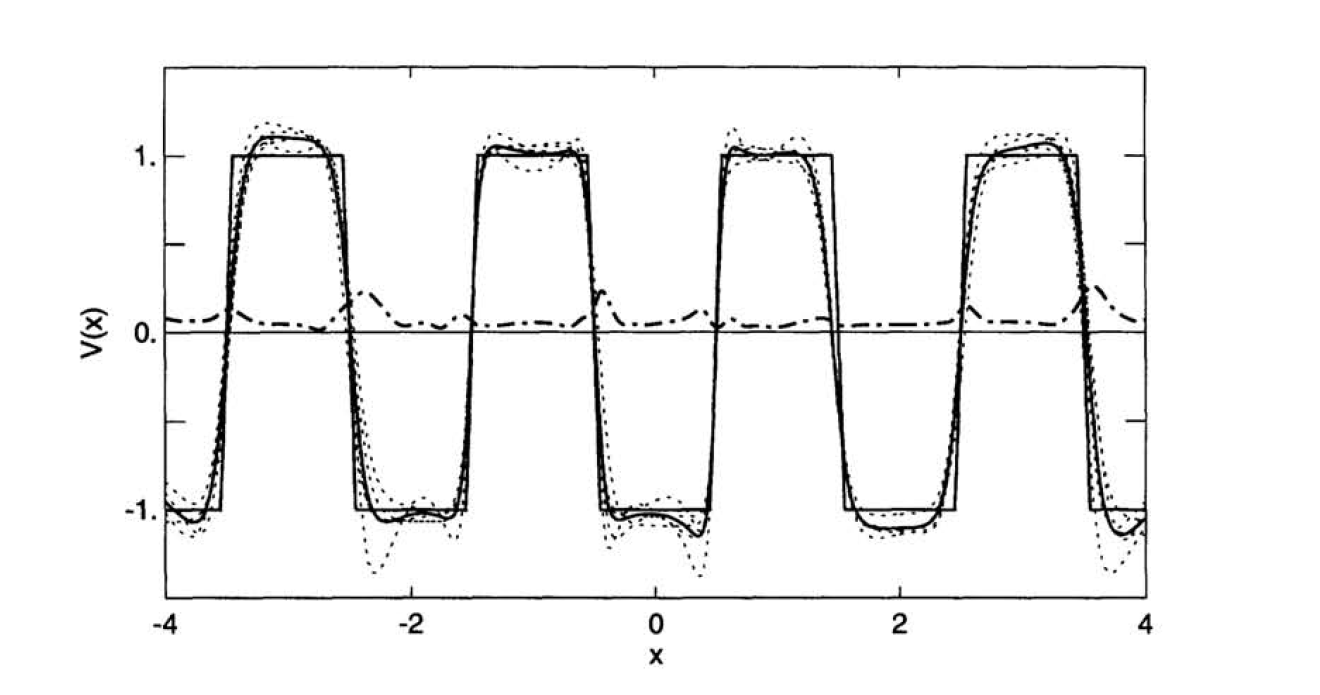
\includegraphics[scale=0.4]{SqWave.png}
   \caption{da inserire}
   \label{SqWavepng}
  \end{figure}
  In figura \ref{GenErrorpng} viene mostrato l'errore generalizzato in funzione della dimensione $K$ dei set per la cross-validation.
  \begin{figure}[h!]
   \centering
   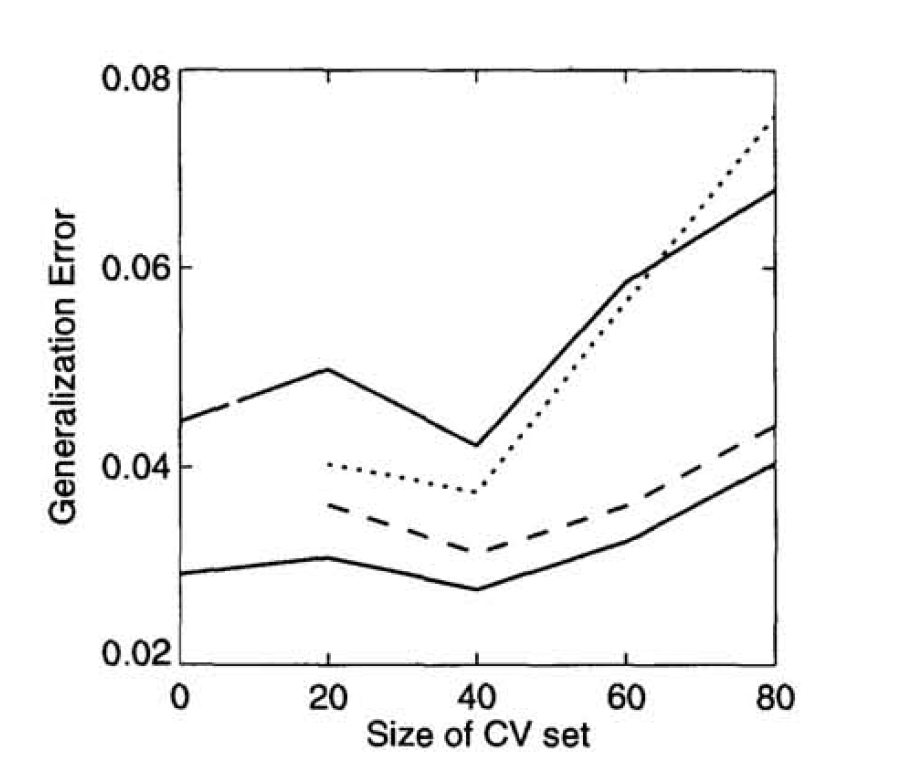
\includegraphics[scale=0.4]{GenError.png} 
   \caption{da inserire}
   \label{GenErrorpng}
  \end{figure}
  Innanzitutto notiamo come l'errore generalizzato sia lo stesso per un set di cross-validation di dimensione 40 o 0. Tuttavia bisogna considerare che sono stati scartati tutti i risultati di ensemble con due o pi\'u reti non convergenti.

  Dopo aver definito pi\'u chiaramente il problema da affrontare, cerchiamone una soluzione. La maggior parte dei lavori precedenti si \'e concentrata sulla combinazione degli output di reti pi\'u performanti o ha indirizzato solo indirettamente il modo in cui generare un buon ensemble di reti, generando casualmente diverse topologie, impostazioni iniziali dei pesi, dei parametri o utilizzando solo una parte del set di training nella speranza di produrre reti che commettano errori per input distinti. Per trovare direttamente un ensemble accurato e diversificato si possono sfruttare gli algoritmi genetici, creando una popolazione iniziale e utilizzando operatori genetici per creare continuamente nuove reti, mantenendo di volta in volta solo l'insieme di reti pi\'u performanti e al contempo pi\'u discordi tra loro. 

  
  In tabella 1 sintetizziamo l'algoritmo utilizzato. Viene creata una popolazione iniziale di reti neurali sottoposta a training. Di seguito si creano nuove reti partendo dalle precedenti utilizzando operazioni ``genetiche'' come mutazioni e crossover. La nuova popolazione viene nuovamente addestrata, ponendo particolare attenzione ad utilizzare gli esempi classificati erroneamente dalla popolazione precedente. Viene quindi associato un punteggio determinato dalla funzione di fitness:
  \begin{equation}
   Fitness_i = Accuracy_i + \lambda Diversity_i = (1-E_i) + \lambda D_i \label{fitness}
  \end{equation}
  con la diversit\'a definita come:
  \begin{equation}
   D_i = \sum \left[ V_i \left(x\right) - \overline{V} \left(x\right) \right]^2. \label{diversity}
  \end{equation}
  
  Definiamo il termine di accuratezza del set di convalida della rete come $A_i = 1-E_i$ e utilizziamo l'equazione \ref{diversity} per calcolare il termine di diversit\'a $D_i$. Quindi normalizziamo separatamente ciascuno dei due termini. Non essendo sempre chiaro con quale valore si debba settare $\lambda$, solitamente ci si basa sulle seguenti regole. Il valore di $\lambda$ non si modifica se l'errore dell'ensemble $\hat{E}$ diminuisce mentre consideriamo nuove reti. Cambia invece se si verifica una delle seguenti: (1) se l'errore della popolazione $\overline{E}$ non sta aumentando e la diversit\'a $D$ sta diminuendo, aumentiamo $\lambda$; (2) se $\overline{E}$ sta aumentando e $\overline{D}$ non decresce, caliamo $\lambda$.
  
  Tabella 1
  \textbf{GOAL:} creare geneticamente un ensemble di reti accurate e diversificate.
  \begin{itemize}
   \item Creare e addestrare la popolazione iniziale di reti.
   \item Finch\'e non si raggiunge un limite di efficacia o di tempo:
   \begin{itemize}
    \item Utilizzare operazioni genetiche per creare nuove reti.
    \item Addestrare le nuove reti utilizzando l'equazione \ref{EnsembleCostFunc}.
    \item Misurare la diversit\'a di ogni rete rispetto alla popolazione corrente (equazione \ref{diversity}).
    \item Normalizzare i termini di accuratezza e diversit\'a delle singole reti.
    \item Cacolare la funzione di fitness in equazione \ref{fitness}.
    \item Aggiornare la popolazione utilizzando le $N$ reti con valore maggiore per la \ref{fitness}.
    \item Corregere $\lambda$ dell'equazione \ref{fitness}
    \item Utilizzare la popolazione attuale di reti come ensemble e combinare gli output delle reti seguendo l'equazione \ref{JudgeWeights}
   \end{itemize}
  \end{itemize}
  Ribadiamo che una rete utile all'ensemble \'e quella che classifica correttamente i maggior numero possibile di casi, mentre pecca principalmente laddove le altre reti classificano correttamente. Ci preoccupiamo di questo aspetto durante la backpropagation moltiplicando la normale funzione di costo per un termine che misura l'errore combinato della popolazione su un determinato esempio:
  \begin{equation}
   Cost = \sum_{k \in T} \left| \frac{t \left(k\right) - \hat{o} \left(k\right)}{\hat{E}} \right|^{\frac{\lambda}{\lambda + 1}} \left[ t\left(k\right) - a\left(k\right) \right]^2 \label{EnsembleCostFunc}
  \end{equation}
  dove $t(k)$ \'e il target e $a(k)$ \'e l'attivazione della rete per l'esempio k nel training set $T$. Si noti che, dato che la nostra rete non \'e ancora un membro dell'ensemble, $\hat{o} (k)$ e $\hat{E}$ non dipendono dalla nostra rete; il nuovo termine \'e perci\'o una costante quando calcoliamo le derivate nella back propagation. Normalizziamo $t(k) - \hat{o} (k)$ dividendo per l'errore dell'ensemble $\hat{E}$ in modo che il valore medio del nostro nuovo termine sia circa 1 indipendentemente dalla correttezza dell'insieme. Ci\'o \'e particolarmente importante con popolazioni particolarmente accurate, pioch\'e $t(k) - \hat{o} (k)$ sar\'a vicino a 0 per la maggior parte degli esempi e la rete verrebbe addestrata solo su un numero esiguo di esempi. L'esponenete $\frac{\lambda}{\lambda + 1}$ rappresenta il rapporto di importanza del termine di diversit\'a nella funzione di fitness. Ad esempio, se $\lambda$ \'e vicino a 0, la diversit\'a non \'e considereta importante e la rete viene addestrata con la consueta funzione di costo; tuttavia se $\lambda$ \'e grande, la diversit\'a \'e cosiderata importante e il nuovo termine nella funzione di costo assume maggiore importanza. Combiniamo le previsioni delle reti prendendo una somma ponderata dell'output di ciascuna rete, dove ogni peso \'e definito come in precedenza. Riportiamo di seguito i risultati ottenuti da David W. Opitz e Jude W. Shavlik.
  L'algoritmo genetico che viene utilizzato per generare nuove topologie di rete \'e l'algoritmo REGENT (Opitz e Shavlik, 1994). REGENT utilizza algoritmi genetici per effettuare ricerche nello spazio delle topologie della rete neurale KN. I KN sono reti le cui topologie sono determinate a seguito della mappatura diretta di un insieme di regole di base che rappresentano ci\'o che attualmente si conosce del problema da afffrontare. KBANN (Towell e Shavlik, 1994), per esempio, traduce un insieme di regole proposizionali in una rete neurale, quindi affina i pesi della rete risultante usando la back-propagation. KNN addestrati, come le reti KBANN, hanno dimostrato di generalizzare frequentemente meglio di molte altre tecniche di apprendimento induttivo come le reti neurali standard (Optiz 1995; Towell e Shavlik, 1994). L'uso di KNN consente di avere reti altamente corrette nell'ensemble; tuttavia, poich\'e ogni rete nell'ensemble \'e inizializzata con lo stesso insieme di regole specifiche del dominio, non ci si aspetta che vi sia un grande disaccordo tra le reti. Un'alternativa da considerare \'e quella di generare casualmente la opolazione iniziale di topologie di rete, poich\'e a volte le regole specifiche del dominio non sono disponibili. \'E stato eseguito l'algoritmo genetico sul set di problemi MAX di NYNEX e su tre problemi del progetto genoma umano che aiutano a localizzare i geni nelle sequenze di DNA. Ognuno di questi domini \'e accompagnato da una serie di regole approssimativamente corrette che descrivono ci\'o che attualmente \'e noto su tale attivit\'a (Opitz 1995, Optiz e Shavlik 1994). Gli esperimenti misurano l'errore del set di test dell'algoritmo genetico su queste attivit\'a. Ogni ensemble \'e composto da 20 reti e gli algoritmi REGENT e ADDEMUP (cos\'i \'e stato chiamato l'algoritmo genetico utilizzato da David W. Opitz e Jude W. Shavlik) hanno considerato 250 reti durante la loro ricerca genetica. La tabella \ref{NoKnowledgeTab} presenta i risultati del caso in cui si creino casualmente la topologia delle reti. La prima riga della tabella \ref{NoKnowledgeTab}, la migliore rete, deriva da una rete neurale a singolo strato in cui, per ogni fold abbiamo addestrato 20 reti contenenti tra 0 e 100 hidden nodes e usato un set di validazione per scegliere la migliore. La riga successiva, il bagging, contiene i risultati dell'esecuzione dell'algoritmo di bagging di Breiman (1994) su reti standard con un unico hidden layer, in cui il numero di hidden nodes viene impostato casualmente tra 0 e 100 per ogni rete. Il bagging \'e un ``bootstrap'', cio\'e un metodo dell'ensemble che forma ogni rete dell'ensemble con una diversa partizione dell'insieme di addestramento. Genera ogni partizione tracciando casualmente, con la sostituzione, N esempi dal set di addestramento, dove N \'e la dimensione del set di addestramento. Breiman (1994) ha dimostrato che il bagging \'e efficace su algoritmi di apprendimento ``instabili'', come le reti neurali, in cui piccole cambiamenti nel set di addestramento comportano grandi cambiamenti nelle previsioni. La riga inferiore della tabella \ref{NoKnowledgeTab}, ADDEMUP, contiene i risultati di una serie di ADDEMUP in cui la popolazione iniziale di 20 individui viene generata casualmente. I risultati mostrano che su questi domini la combinazione dell'output di pi\'u reti addestrate di generalizza meglio rispetto al tentativo di scegliere la rete singola rete migliore. Mentre la tabella \ref{NoKnowledgeTab} mostra la potenza degli insiemi di reti neurali, la tabella \ref{KnowledgeTab} mostra la capacit\'a di ADDEMUP di utilizzare le conoscenze a priori del problema. La prima riga della tabella \ref{KnowledgeTab} contiene i risultati di generalizzazione dell'algoritmo KBANN, mentre la riga successica, KBANN-bagging, contiene i risultati dell'ensemble in cui ogni singola rete \'e la rete KBANN addestrata su una diversa partizione dell'insieme di  addestramento. Sebbene ciascuna di queste reti inizi con la stessa topologia e impostazione di peso iniziali ``grande'' (i pesi risultanti dalla conoscenza specifica del dominio), piccoli cambiamenti nel set di allenamento producono ancora cambiamenti significativi nelle previsioni. Si noti inoltre che su tutti i set di dati, il bagging KBANN \'e migliore dell'esecuzione del bagging su reti generate casualmente (bagging della tabella \ref{NoKnowledgeTab}). La riga successiva, REGENT-combined, contiene i risultati della semplice combinazione, usando l'equazione \ref{JudgeWeights}, le reti nella popolazione finale di REGENT. ADDEMUP, l'ultima riga della tabella \ref{KnowledgeTab}, differisce principalmente da REGENT-combined in due modi: (1) la sua funzione di fitness (equazione \ref{fitness} ) tiene conto della diversit\'a piuttosto che della sola precisione della rete e (2) allena le nuove reti enfatizzando gli esempi errati dell'ensemble attuale. Pertanto, il confronto di ADDEMUP con REGENT-combined aiuta a testare direttamente la diversit\'a di ADDEMUP, anche se i risultati aggiuntivi riportati in Opitz (1995) mostrano che ADDEMUP ottiene gran parte del suo miglioramento dalla sua funzione di fitness. Ci sono due ragioni principali per cui si ritiene che i risultati di ADDEMUP nella tabella \ref{KnowledgeTab} siano particolarmente incoraggianti: (1) confrontando ADDEMUP con REGENT-combined, testiamo esplicitamente la qualit\'a dell'euristica e si dimostra la loro efficacia e (2) ADDEMUP \'e in grado di utilizzare efficacemente le conoscenze di base per ridurre l'errore delle singole reti nel suo insieme, pur essendo in grado di creare abbastanza diversit\'a tra di loro in modo da migliorare la qualit\'a complessiva dell'ensemble. 
  
  \begin{table}[h]\caption{Standard neural networks (no domain-specific knowledge used)} \label{NoKnowledgeTab}
   \centering
   \begin{tabular}[h]{|l|c|c|c|c|}
    \hline
    & Promoters & Splice Junction & RBS & MAX \\ \hline
   best-network & 6.6\% & 7.8\% & 10.7\% & 37.0\% \\ 
   bagging & 4.6\% & 4.5\% & 9.5\% & 35.7\% \\
   ADDEMUP & 4.6\% & 4.9\% & 9.0\% & 34.9\% \\ \hline
   \end{tabular}
  \end{table}
  
  \begin{table}[h]\caption{Knowledge-based neural networks (domain-specific knowledge used)} \label{KnowledgeTab}
   \centering
   \begin{tabular}[h]{|l|c|c|c|c|}
    \hline
       & Promoters & Splice Junction & RBS & MAX \\ \hline
    KBANN & 6.2\% & 5.3\% & 9.4\% & 35.8\% \\ 
    KBANN-bagging & 4.2\% & 4.5\% & 8.5\% & 35.6\% \\
    REGENT-combined & 3.9\% & 3.9\% & 8.2\% & 35.6\% \\
    ADDEMUP & 2.9\% & 3.6\% & 7.5\% & 34.7\% \\ \hline
   \end{tabular}
  \end{table}
 
\end{document}

